\subsection{Astrobiology System}
\label{sec:AstrobiologySystem}

\subsubsection{Design and Operation}
The collection assembly will be designed as a single mechanized enclosure as shown below. The rotating arm will be raised out of the collection container and began rotating once float altitude has been reached. The raising of the rotating arms will be done by a L-16 linear servo motor. The rotation of the filter arm will be provided by the rotational motor mounted onto the filter arm. The lid on the top of the linear servo will seal the clean box during ascent and descent. The  Fluropore Membrane filters will be mounted on the ends of the rotating arm. The arms will spin at 80 RPM for the duration of float conditions. In theory, the sampled volume will be the cross-sectional area of each filter multiplied by the distance the payload travels, which results in a far greater sampled volume than the 0.03 liters per minute sampling of the pumps from the previous flight.\cite{SORA2} When it is time for the payload to descend, a command will be sent to retract the rotating mechanism back into the clean box. The fluropore filters on the rotation arm will be compared to the ones on mounted on the linear servo as shown in the figure below. Background samples will be taken using the same fluropore membrane filters and will sample the various places the payload will be, such as the UH lab room, the clean room used for sterilization and the Fort Sumner launch site. 

\begin{figure}[!h] 
	\begin{center}
		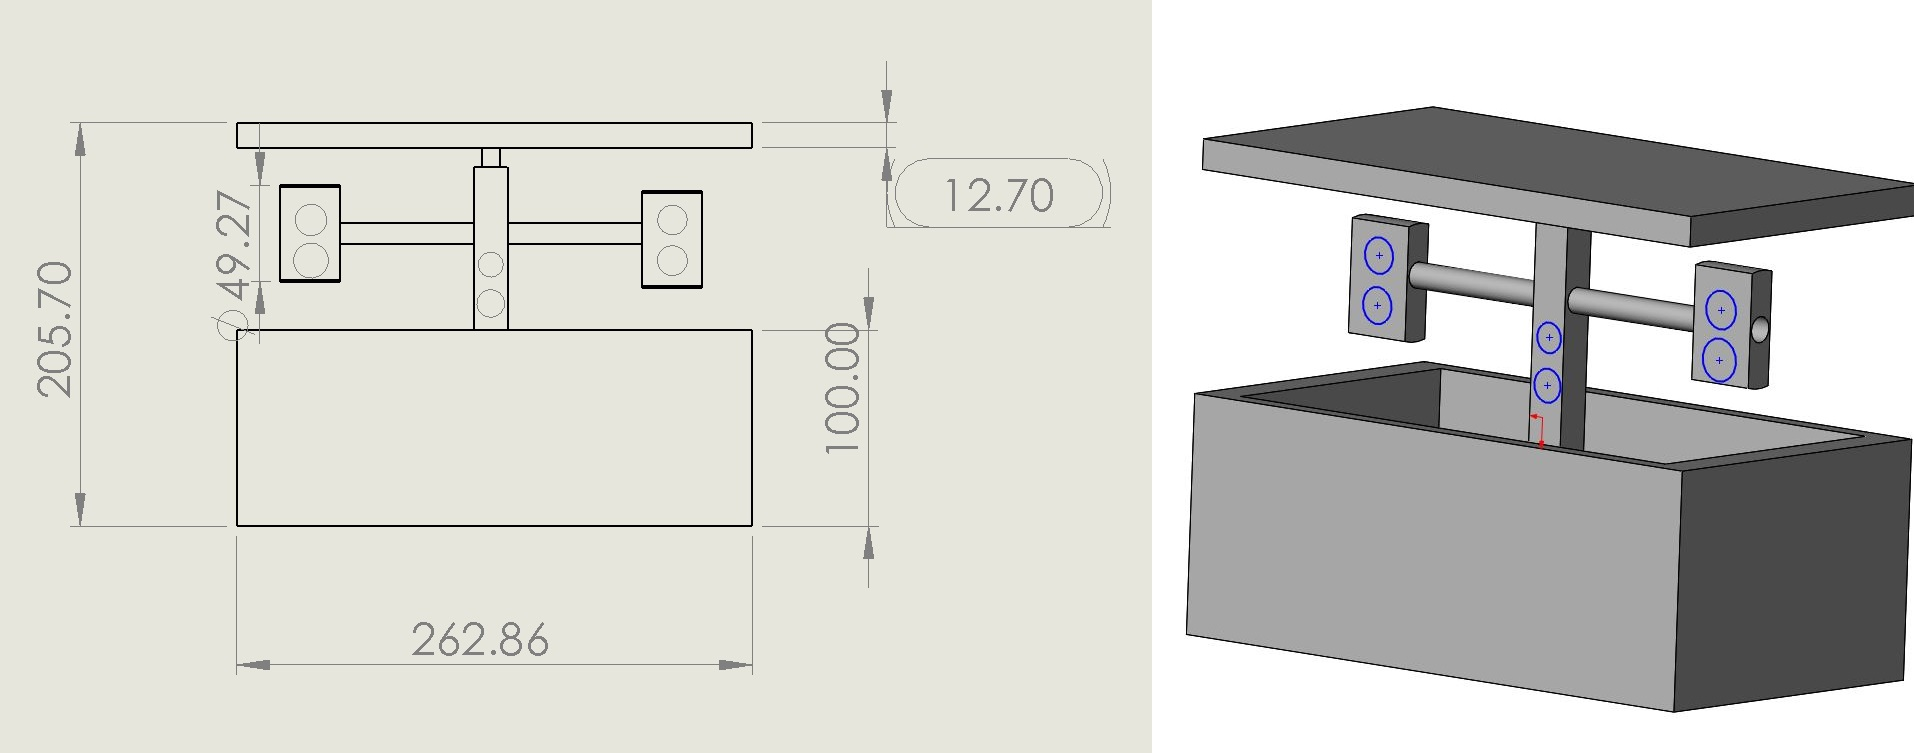
\includegraphics[width=\linewidth]{Figures/T-Arm.jpg}
		\caption{Cross-section view of the clean box with the extended rotating arm. \bf All numbers are in millimeters}
		\label{fig:AstroBox}
	\end{center}
\end{figure} 
%\subsection{Astrobiology Methods}
%\label{sec:Astrobiology Methods}
\subsubsection{Pre-Flight Preparation}
The rotating arm mechanism will be tested in low pressure and in various mounting positions. Once it is certain that the arm functions in the intended conditions during flight. We will take it to the clean room to be sterilized.  

The clean box that houses the arm  will autoclaved. All tools used in the assembly of the clean box will either be autoclaved or soaked in a \SI{70}{\percent} ethanol solution inside of a clean room. Each person who enters the clean room will be garbed in a lab coat, goggles, hair net and latex gloves after thoroughly washing their hands in a \SI{70}{\percent} ethanol solution.All wires within in the box will be soaked in the \SI{70}{\percent} ethanol solution and the rotating arm mechanics will be powered on and retracted the box. The box will then be integrated into the payload. 
\subsubsection{Post-Flight Procedures}

Once the payload is retrieved, the intact clean box needs to be removed and placed inside of a cooler with ice to be then transported to The University of Houston and placed in cold storage at \SI{4}{\celsius}. All equipment used in the filtration process will be either autoclaved or taken from previously unopened sanitized packaging. The autoclaved, pre-sanitized items and the clean box will then be washed in a \SI{70}{\percent} ethanol solution before they are placed inside a SterilGARD e3 Class II Biological Safety Cabinet (the Cabinet). The cabinet has a laminar flow air barrier and UV lights built into the ceiling for decontaminating the workspace prior to use.The Fluropore Membrane filters from the clean box and the backgeound samples will be processed through a DNA extraction kit and the remaining sample fluid will be stored in the cold storage for in-house 16S ribosomal RNA sequencing through the University of Houston sequencing team.  

